\documentclass[tikz,border=2pt]{standalone}
\usepackage{amsmath,amssymb}
\usepackage{pgfplots}
\pgfplotsset{compat=1.18}
\usetikzlibrary{arrows.meta}

\begin{document}
% Graphs {(x, f(x))} of six functions: a line, a parabola, a cubic, the hyperbola 1/x (two
% branches), the square root (x >= 0) and the exponential.
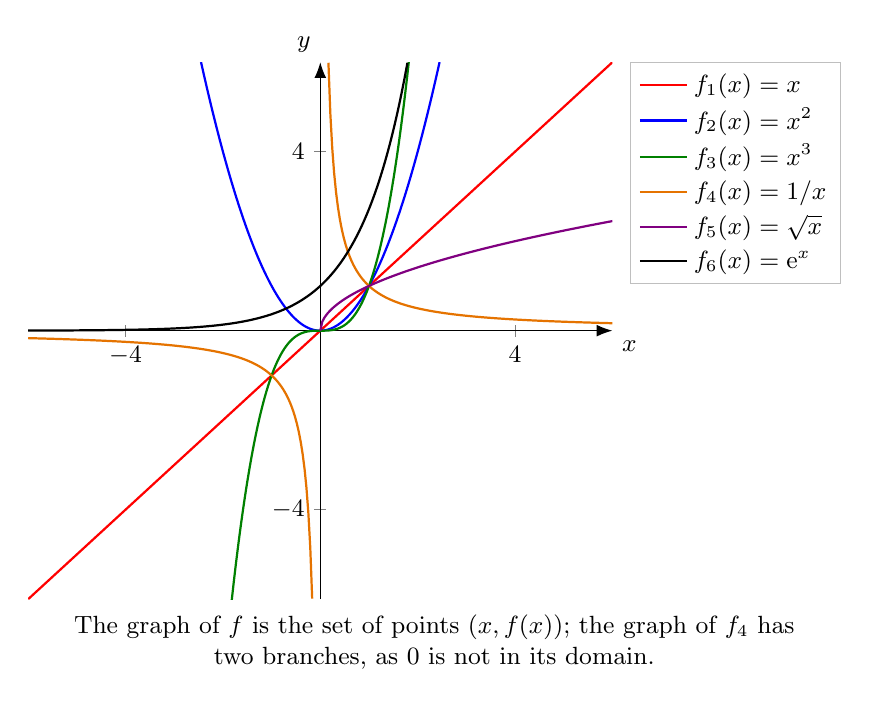
\begin{tikzpicture}[every node/.style={font=\small}]
	\begin{axis}[
		width=9cm, height=8.4cm,
		axis lines=middle, axis line style={-{Latex[length=2mm]}},
		xmin=-6, xmax=6, ymin=-6, ymax=6,
		xtick={-4,4}, ytick={-4,4},
		tick label style={font=\small},
		xlabel={$x$}, ylabel={$y$},
		xlabel style={below right}, ylabel style={above left},
		samples=150,
		legend pos=outer north east, legend cell align={left},
		legend style={font=\small, draw=gray!50, fill=white}
		]
		\addplot[red, thick, domain=-6:6] {x};
		\addlegendentry{$f_1(x)=x$}
		\addplot[blue, thick, domain=-2.45:2.45] {x^2};
		\addlegendentry{$f_2(x)=x^2$}
		\addplot[green!50!black, thick, domain=-1.82:1.82] {x^3};
		\addlegendentry{$f_3(x)=x^3$}
		\addplot[orange!90!black, thick, domain=0.167:6] {1/x};
		\addlegendentry{$f_4(x)=1/x$}
		\addplot[orange!90!black, thick, domain=-6:-0.167, forget plot] {1/x};
		\addplot[violet, thick, domain=0:6] {sqrt(x)};
		\addlegendentry{$f_5(x)=\sqrt{x}$}
		\addplot[black, thick, domain=-6:1.79] {exp(x)};
		\addlegendentry{$f_6(x)=\mathrm{e}^x$}
	\end{axis}
	\node[anchor=north, align=flush center, text width=9.6cm] at ([yshift=-2pt]current bounding box.south) {The graph of $f$ is the set of points $(x,f(x))$; the graph of $f_4$ has two branches, as $0$ is not in its domain.};
\end{tikzpicture}
\end{document}
